\documentclass{book}
/Users/jmft2/Documents/writing/preamble.tex
\numberwithin{equation}{section}

\title{Fluid Dynamics of the Environment}
\author{
    Lecturers: Stuart Dalziel, Andy Woods and Nathalie Vriend \\ 
Notes by Jonathan Michael Foonlan Tsang}

\begin{document}
\maketitle

These notes are primarily based on the course as it was given in Michaelmas 2014
by Stuart Dalziel and Nathalie Vriend, or on the Michaelmas 2015 version by
Dalziel, Vriend and Woods. The headings in the table of contents reflect
the official structure of the course, except in \S\ref{section-nmv}. An asterisk
denotes a section which was either not lectured or not examinable in 2014, but
this will not necessarily be true for other years. 

The contents of these notes are \textit{not} official.

In the past, this course was known as `Geophysical and Environmental Fluid
Dynamics', `Environmental Fluid Dynamics', or a variety of other names.

\tableofcontents

\newpage
\section{Internal gravity waves}
\subsection{The minimal mathematics version}

In a stably stratified fluid, consider a parcel of fluid. If the parcel is raised from its original position, then it will be heavier than the surrounding fluid, and will sink back down. If it is lowered, then buoyancy will push it back up. Thus density differences provide a restoring force to a parcel displaced vertically. 

Let $\rho(z)$ be the density of the fluid, with $z$ vertically upwards so that $\dod{\rho}{z} < 0$. If the parcel has volume $V$ and is displaced vertically by a height $H$, then the density difference between the parcel and the surrounding fluid is 
\begin{equation}
	\Delta\rho = \dod{\rho}{z} H
\end{equation}
and the downwards force on the parcel is therefore
\begin{equation}
	F = gV\Delta\rho = gV\dod{\rho}{z}H
\end{equation}
Meanwhile, the mass of the particle is 
\begin{equation}
	m = \rho V
\end{equation}
and so Newton's law $F = ma$ gives the acceleration
\begin{equation}
	a = \frac{g}{\rho}\dod{\rho}{z} H
\end{equation}
which is in the opposite direction to the displacement.

Assume that the fluid is \textit{Boussinesq}, so that density differences are small compared to a reference density $\rho_0$, and fluid accelerations are small compared to gravity. Then we make the approximation $\rho\approx\rho_0$ except when densities are multiplied by gravity. We define the \textit{buoyancy frequency} (or \textit{Brunt-V\"ais\"al\"a frequency}) $N$, such that
\begin{equation}
	N^2 = -\frac{g}{\rho_0}\dod{\rho}{z}.
\end{equation}
Then 
\begin{equation}
	a = -N^2 H
\end{equation}
so parcels of fluid execute oscillations with frequency $\omega = N$.

In the oceans, $N \approx 10^{-2}\mathrm{s^{-1}}$.

The above argument is not quite valid, because we cannot ignore continuity: we cannot simply displace a parcel of fluid without displacing some other fluid around it. Rather, we should consider displacing an entire slab of fluid and making it oscillate in its plane. But the same argument works.

Suppose a slab makes an angle $\theta$ to the vertical and is displaced by $d$ in that direction. Then the displacement in the vertical direction is $d\cos\theta$. A similar argument shows that the slab will execute oscillations with frequency
\begin{equation}
	\omega = N\cos\theta
\end{equation}

\subsection{A more rigorous derivation}

We can derive the above more rigorously by starting from the governing equations of an incompressible inviscid fluid:
\begin{align}
	\divg\bs{u} &= 0\\
	\rho_t + \divg(\rho\bs{u}) &= 0\\
	(\rho\bs{u})_t +\divg(\rho\bs{u}\bs{u}) &= -\grad p + \rho\bs{g} 
\end{align}
which may also be written as 
\begin{align}
	\divg\bs{u} &= 0\\
	\rho_t + \bs{u}\cdot\grad\rho &= 0\\
	\rho (\bs{u}_t +\bs{u}\cdot\grad\bs{u}) &= -\grad p + \rho\bs{g}.
\end{align}
We perturb about the stationary stratified state, writing
\begin{align}
	\rho &= \bar{\rho}(z) + \rho' \\
	p &= \bar{p}(z) + p' 
\end{align}
and assume that the primed quantities and $\bs{u}$ are small. Then linearising the governing equations gives
\begin{align}
	\divg\bs{u} &= 0\\
	\dod{\bar{p}}{z} &= -g\bar{\rho} \\
	\rho_t &= -w\dod{\bar{\rho}}{z} \\
	\bar{\rho} \bs{u}_t &= -\grad p' - g\rho'\bs{e}_z. \label{govlin-mom}
\end{align}
For a Boussinesq fluid, $\rho\approx\rho_0$ except when multiplied by $g$, so (\ref{govlin-mom}) becomes
\begin{align}
	\bs{u}_t = -\frac{1}{\rho_0}\grad p' - \frac{g}{\rho_0} \rho' \bs{e}_z. \label{govlinbous-mom}
\end{align}
Take $\divg$(\ref{govlinbous-mom}) and use $\divg\bs{u} = 0$ to get
\begin{equation}
	\grad^2p' = -g\dpd{\rho'}{z}
\end{equation}
and then take $\grad^2$ of the $z$-component of (\ref{govlinbous-mom}) to get 
\begin{equation}
	\grad^2 w_t = -\frac{g}{\rho_0} (\rho'_{zz} - \grad^2 \rho')
\end{equation}
Differentiating with respect to time and using the equation for $\rho'_t$ gives
\begin{align}
	\grad^2w_tt &= \frac{g}{\rho_0} \left(\grad^2 - \dpd[2]{}{z}\right) (w\bar{\rho}_z) \\
			&\approx N^2 \left(\dpd[2]{}{z} - \grad^2\right) w
\end{align}
where the approximation applies for a Boussinesq fluid.

For normal mode perturbations of the form
\begin{equation}
	w = \hat{w}\exp(i(\bs{k}\cdot\bs{x}-\omega t))
\end{equation}
where $\bs{k} = (k,l,m)$, we get the dispersion relation
\begin{equation}
	\omega^2 = N^2 \frac{k^2+l^2}{k^2+l^2+m^2}
\end{equation}

How do we relate this to the argument with slabs, and recover $\omega = N\cos\theta$? We note that the slabs that we considered were lines of constant phase, i.e. of constant $\bs{k}\cdot\bs{x}$. So $\bs{k}$ is perpendicular to the slab. Hence if the slab makes an angle $\theta$ with the upwards vertical, then $\bs{k}$ makes an angle $\theta$ with the horizontal, and so
\begin{equation}
	\cos\theta = \frac{k^2+l^2}{k^2+l^2+m^2}
\end{equation}
as required. 

\subsection{Wave velocities}

From the dispersion relation, we obtain the phase and group velocities in the usual way:
\begin{align}
	\bs{c}_p &= \frac{\omega}{|\bs{k}|} \hat{\bs{k}} \\
		&= \frac{N}{k}\cos\theta \hat{\bs{k}} \\
		&= N \sqrt{\frac{k^2+l^2}{k^2+l^2+m^2}} (k,l,m)
\end{align}
and
\begin{align}
	\bs{c}_g &= \dpd{\omega}{\bs{k}} \\
		&= -N \sin\theta \dpd{\theta}{\bs{k}}\\
		&=\frac{N}{|\bs{k}|^3 \sqrt{k^2+l^2}} (km^2,lm^2,-(k^2+l^2)m)
\end{align}

Note that 
\begin{equation}
	\bs{c}_p\cdot\bs{c}_g = 0
\end{equation}
so the phase and group velocities are perpendicular; and note that the group and phase velocities have $z$-components in opposite directions. See figure \ref{fig:igw-wave-vels}.

The phase velocity is the velocity at which crests move, or more abstractly the velocity at which phase is advected. The group velocity is the velocity with which wavepackets propagate, and can be interpreted as a rate and direction of energy transfer. The group velocity makes an angle $\theta$ with the vertical. 

\begin{figure}
\begin{center}
	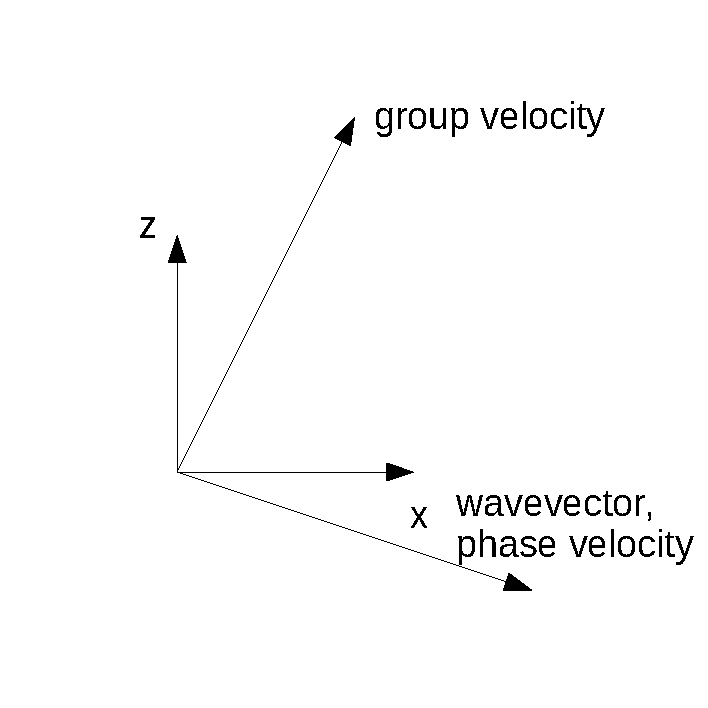
\includegraphics[width=8cm]{igw-wave-vels.pdf}
	\caption{The geometric relationship between phase velocity, group velocity and wavevector.}
	\label{fig:igw-wave-vels}
\end{center}
\end{figure}

\subsection{Motion of fluid particles}

If $\bs{u} = (u,0,w)$ and 
\begin{align}
	u&=\hat{u} \exp(i(\bs{k}\cdot\bs{x} - \omega t)) \\
	w&=\hat{w} \exp(i(\bs{k}\cdot\bs{x} - \omega t)) \\
\end{align}
then $\divg\bs{u}=0$ gives
\begin{equation}
	\hat{u} = -\frac{m}{k}\hat{w}
\end{equation}
which tells us that fluid particles oscillate parallel to the group velocity and perpendicularly to the wavevector. We can obtain the displacements by integrating with respect to time, or equivalently by dividing by $-i\omega$. 

\subsection{Equipartition of energy}

Dotting (\ref{govlinbous-mom}) with $\bs{u}$ and some manipulation gives us
\begin{equation}
	\dpd{}{t}\left(\frac{1}{2}\rho_0 \bs{u}^2 + \frac{1}{2}\frac{g^2}{\rho_0N^2}\rho'^2\right) + \divg(p'\bs{u}) = 0,
\end{equation}
the equation of conservation of energy. We identify $ \frac{1}{2}\rho_0 \bs{u}^2 $ as kinetic energy density and $\frac{1}{2}\frac{g^2}{\rho_0N^2}\rho'^2$ as potential energy density. (Energy density is energy per unit volume.)

For normal modes, we can calculate time-averages, and find that 
\begin{equation}
\langle\text{kinetic energy density}\rangle = \langle\text{potential energy density}\rangle
\end{equation}
%TODO

\subsection{Oscillating cylinders}
\subsection{Reflexions}
\subsubsection{Properties of reflected beams}

\begin{figure}
\begin{center}
	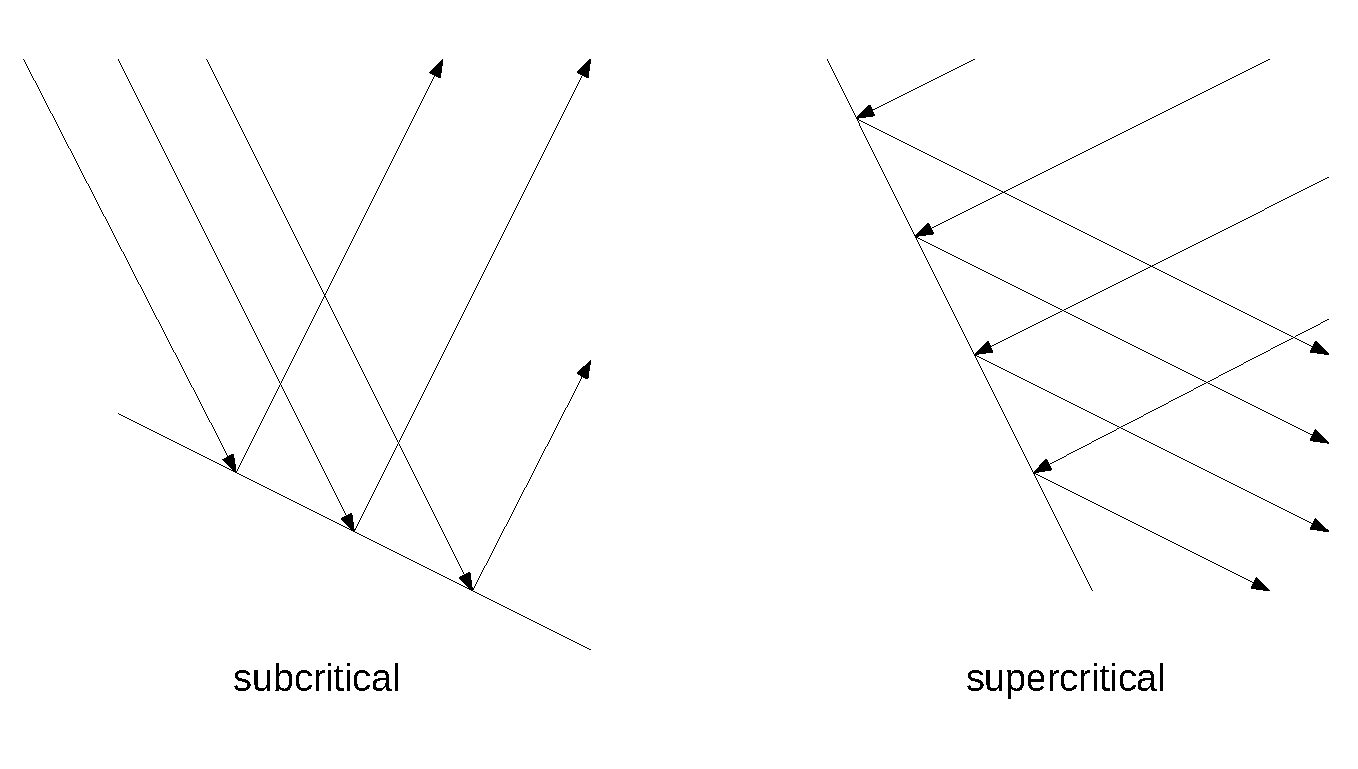
\includegraphics[width=14cm]{super-and-sub-critical.pdf}
	\caption{Super- and sub-critical reflexions.}
	\label{fig:supersubcrit}
\end{center}
\end{figure}


At a boundary, the normal velocity component must be continuous. For a rigid stationary boundary, this means that the normal velocity component must vanish.

Suppose $z=0$ is a rigid stationary boundary, with a plane wave incident from $z>0$. What is the reflected wave? We have 
\begin{align}
	w &= w_I + w_R \\
	w_I &= \hat{w}_I \exp(i(\bs{k}_I\cdot\bs{x} - \omega t)) \\
	w_R &= \hat{w}_I \exp(i(\bs{k}_R\cdot\bs{x} - \omega t));
\end{align}
the two waves must have the same $\omega$ and $k_I = k_R$; the boundary condition gives $\hat{w}_I + \hat{w}_R = 0$. And causality implies that $m_R = -m_I$. 

When a plane wave reflects off a flat boundary which is not horizontal, then the incident and reflected waves make the same angle (but reflected) with the vertical or horizontal, so that they have the same $\omega = N\cos\theta$. (Note that for IGWs, $\theta$ is the angle between a wave's direction and the vertical.) In general, the angle of incidence and angle of reflexion are not equal. Depending on how the angle of the incident wave compares with the slope of the boundary, one of two things may happen: see Figure \ref{fig:supersubcrit}. 

From Figure \ref{fig:supersubcrit} we can see that reflexions change the wavenumber of the wave and can act to focus or defocus the rays, depending on direction. Let $\alpha$ be the angle that the plane boundary makes with the vertical. We define the quantity 
\begin{equation}
	\gamma  =  \frac{\sin(\alpha-\theta)}{\sin(\alpha+\theta)}
\end{equation}
to characterise the focusing power of a reflexion. 

After a lot of manipulation, we can show that focusing reflexions change the amplitude and wavenumber according to
\begin{align}
	k_R  &= \gamma k_I \\
	A_R &= \gamma A_I 
\end{align}
and that defocusing reflexions have the opposite effect:
\begin{align}
	k_R  &= \gamma^{-1} k_I \\
	A_R &= \gamma^{-1} A_I.
\end{align}

\subsubsection{Energy density upon reflexion}

The energy density per unit wavelength is 
\begin{equation}
	\tilde{E} \sim \lambda A^2.
\end{equation}
After a focusing reflexion, $\lambda$ is divided by $\gamma$ but $A$ is multiplied by $\gamma$, so $\tilde{E}$ is multiplied by $\gamma$. Hence the energy density per wavelength is increased after a focusing reflexion. 

The energy density per unit length is 
\begin{equation}
	\hat{E} = \frac{1}{\lambda} \tilde{E}
\end{equation}
and so $\hat{E}$ is multiplied by $\gamma^2$ after a focusing reflexion.

\subsubsection{Subcritical and supercritical reflexions}

In a subcritical reflexion, the boundary has a shallower slope than the wave ($\theta < \alpha$), and the vertical propagation of the wave is reversed by the reflexion. The horizontal direction of propagation is maintained.

In a supercritical reflexion, $\theta > \alpha$ and the vertical direction of propagation is maintained but the horizontal direction is reversed. 

When $\theta$ and $\alpha$ are very similar, then $\gamma$ becomes very large. So waves will have very large amplitudes, and nonlinear effects and viscosity become important. 

\subsection{Ray tracing}

Since the frequency is preserved upon reflexion, the angle to the vertical $\theta$ is conserved, so waves tend to propagate along well-defined rays. Depending on the shape of the domain and its boundaries, repeated reflexions can lead to trapping, to amplitudes increasing, and eventually to wave-breaking. Nonlinear effects become important if the amplitude of waves is increased sufficiently.

We must take note of causality to determine which direction is appropriate.

\subsection{Wave attractors}
\subsubsection{Rectangular basins}
\subsubsection{Trapezoidal basin}
\subsubsection{More complex geometries}
\subsubsection{Energy spectrum for attractor}

\subsection{Decay along a beam}

\subsection{Reflexions from rough topology}

\subsubsection{Subcritical reflexion from a sinusoidal}
\subsubsection{Supercritical reflexions from a sinusoidal}

\subsection{Non-linear stratification}

If $N$ is not constant but varies with $z$ (say), then waves will not follow straight paths but will refract. If $N$ varies very slowly with $z$, over lengthscales much larger than a wavelength, then the WKB method can be used to find the trajectory of a wave. We use the fact that $\omega = N(z)\cos\theta$ is constant along any beam to determine $\theta$, the angle between the beam and the vertical. 



\subsection{Leewaves}

When a medium flows past an obstacle and waves are formed in the wake, it is possible to get standing waves (also known as stationary waves). When standing IGWs occur in the atmosphere as a wind flows past obstacles such as mountains, these are known as leewaves.

\subsubsection{Kelvin ship waves}

As an aside to introduce standing waves, we consider a ship moving with velocity $\bs{U} = U\bs{e}_x$ in deep water. The surface waves have a dispersion relation
\begin{equation}
\omega^2 = g|\bs{k}|
\end{equation}
and phase
\begin{equation}
	\phi = \bs{k}\cdot\bs{x} - \omega t.
\end{equation}
Let $\bs{x}'$ denote a position vector relative to the ship, so that $\bs{x}' = \bs{x} - \bs{U}t$. Then
\begin{equation}
	\phi = \bs{k}\cdot\bs{x}' + (\bs{k}\cdot\bs{U} - \omega) t.
\end{equation}
Hence waves that are stationary in the frame of the ship have
\begin{align}
	\bs{k}\cdot\bs{U} &= \omega \\
	U\cos\theta &= |\bs{c}_g|
\end{align}
where, in this section, $\theta$ is the angle between $\bs{U}$ and $\bs{k}$. 

For these waves, $\bs{c}_g$ and $\bs{c}_p$ are parallel, and $|\bs{c}_g| = \frac{1}{2} |\bs{c}_p| = \frac{1}{2}U\cos\theta$. This is the speed at which wave packets travel. Some geometry then tells us the shape that these waves make behind the ship.

In shallow water, surface waves are not dispersive and such stationary waves are not seen.

\subsubsection{Extended range of hills}

Now we consider leewaves, i.e. stationary atmospheric IGWs as a wind of speed $U$ flows over a sinusoidal mountain range which has wavelength $\lambda$ and so topographical wavenumber $k_T = 2\pi/\lambda$. 

An observer in the frame of the mountains sees the leewaves as having constant phase. 

\subsubsection{Causality}

\subsection{Shear flows}
\subsubsection{Sheared base state}
\subsubsection{Ray tracing in a shear flow}
\subsubsection{*Three-dimensional forcing}
\subsubsection{*Effect of viscosity}
\subsubsection{*Blocking}

\subsection{Columnar modes}
\subsection{*Stokes drift in internal waves}
\subsection{Resonant triads}

\newpage
\section{Turbulence primer}

Most environmental and geophysical flows occur at high Reynolds numbers. At high
Reynolds numbers, laminar solutions to the Navier-Stokes equations are unstable,
and the flows are turbulent. 

\subsection{Basics of turbulence}

Throughout this and the next section, assume that the density $\rho$ is constant
and uniform.

\subsubsection{What is turbulence?}

Although there is no simple definition for turbulence, turbulent flows can be
characterised by a few properties:
\begin{itemize}
    \item Turbulent flows are dominated by inertia, since $\mathrm{Re}\gg1$.
        Viscosity plays a small (but crucial) role.
    \item Turbulent flows are vortical, not irrotational. However, vortical
        flows need not be turbulent.
    \item Turbulent flows involve a range of length scales. Vortices exist at
        both large and small length scales: ``Big whorls have little whorls,
        which feed on their velocity, // And little whorls have lesser whorls,
        and so on to viscosity.'' ---Lewis Richardson.
\end{itemize}
Turbulent flows are unpredictable and simulating them numerically may be difficult as they may be numerically unstable. However, it may be possible to predict certain statistics of the flow, such as the behaviour of the mean flow or mean pressure (noting that fluctuations about these means may be great). Some features of turbulence can be shown to be universal.

Lewis Richardson's couplet describes the two processes at work in a turbulent flow. \textit{Vortex stretching} is responsible for creating small vortices out of large ones, while \textit{energy dissipation} causes small vortices to decay.

\subsubsection{Vortex stretching}

Vortex stretching is the main process by which energy is transferred from large scales to smaller scales.

Taking the curl of the Navier-Stokes equation gives the \textit{vorticity equation}:
\begin{equation}
    \pd{\omega}{t} + \bs{u}\cdot\grad\bs{\omega} 
     = \bs{\omega}\cdot\grad\bs{u} + \nu\grad^2\bs{\omega}
 \label{vorticity-eqn}
\end{equation}
The second term on the RHS of (\ref{vorticity-eqn}) means that vorticity is diffused with diffusion constant $\nu$. This is a minor effect in flows with $\mathrm{Re}\gg1$. The first term means that when a parcel of fluid is stretched into a column, its vorticity increases and becomes aligned with the column. Thus stretching a vortex takes energy to a smaller scale. However, if the vortex column is compressed, not nearly as much energy is taken back to the large scale, since the compression in general de-aligns the vorticity vector and the column.

\subsubsection{Energy dissipation: Kolmogorov's theory (1941)}

We know that energy is dissipated in a fluid at a rate
\begin{equation}
	\Delta = \int_V\mu|\grad\bs{u}|^2dV
\end{equation}
(or expressed in terms of the strain rate tensor, using $|\grad\bs{u}|^2=2e_{ij}e_{ij}$). In a volume with characteristic length $L$, 
\begin{equation}
	\Delta \sim L^3 |\grad\bs{u}|^2.
\end{equation}
For a laminar flow with characteristic velocity $U$ in a box with sides $L$, $|\grad\bs{u}|\sim U/L$ and so
\begin{equation}
\Delta \sim \mu\frac{U^2}{L^2}L^3 = \mu U^2 L.
\end{equation}  
However, for a turbulent flow, the energy dissipation is much faster than this, because the velocity gradients are over much smaller distances, and so $|\grad\bs{u}|\gg U/L$. 

Although the large-scale structure of the flow might have characteristic lengthscale $L$, the small-scale structure of the flow should be described by another lengthscale $\eta$, called the \textit{Kolmogorov length scale} or the \textit{Kolmogorov microscale}. This is the lengthscale at which the effects of vortex stretching and dissipation balance each other.

To summarise: The flow is externally driven (continually or initially) at the lengthscale $L$, energy cascades to smaller lengthscales by vortex stretching; viscosity acts more and more strongly at these smaller lengthscales. Eventually, energy cascades down to the lengthscale $\eta$ and proceeds no more.

Let $\bs{U}(\bs{k})$ be the Fourier transform of the velocity $\bs{u}(\bs{x})$, using the normalisation
\begin{equation}
    \bs{U}(\bs{k}) = \frac{1}{\sqrt{2\pi}} \int_V \bs{u}(\bs{x}) e^{-i\bs{k}\cdot\bs{x}} d\bs{x}.
\end{equation}
Let 
\begin{equation}
    E(\bs{k}) = \frac{1}{2}\rho\bs{U}(\bs{k})\cdot\bs{U}(\bs{k})*
\end{equation}
be the energy density spectrum. (In defining these Fourier transforms, we are assuming that $\rho$ is constant and uniform.) The total kinetic energy is
\begin{equation}
    KE = \int E(\bs{k}) d\bs{k}
\end{equation}
with the integral taken over wavenumber space. For isotropic turbulence, $\bs{U}$ and $E$ depend only on the magnitude $k=|\bs{k}|$. 

Since density is constant, we will find it convenient to rewrite the above expressions without $\rho$, so that the dimension $M$ may be set to $1$. We therefore work with the energy dissipation rate 
\begin{equation}
    \epsilon = \int_V\nu|\grad\bs{u}|^2dV
\end{equation}
which has dimensions $L^2 T^{-3}$, and with the energy spectrum
\begin{equation}
    E(k) = \frac{1}{2}\bs{U}(k)\cdot\bs{U}(k)*
\end{equation}
which has dimensions $L^3 T^{-2}$. We write 
\begin{equation}
    KE = \int E(k) dk
\end{equation}
for the kinetic energy per unit mass, with dimensions $L^2 T^{-2}$.

Kolmogorov made two hypotheses about isotropic turbulent flows. These hypotheses allow us to make progress by dimensional analysis, but they do not follow from first principles, and their predictions must be verified experimentally.

\paragraph{First hypothesis} The rate of dissipation of energy (per unit density), $\epsilon$ (dimensions $L^2T^{-3}$), depends only on viscosity $\nu$ (dimensions $L^2T^{-1}$) and on the microscale $\eta$. In particular, $\epsilon$ and $\eta$ are not to depend on the large lengthscale $L$.

By dimensional analysis, this hypothesis allows us to construct $\eta$:
\begin{equation}
    \eta = (\nu^3 / \epsilon)^{1/4}
\end{equation}

Note that in a system in dynamic equilibrium, the rate of dissipation of energy is equal to the rate of energy input.
\footnote{We can have a dynamic equilibrium, but not a static one, since turbulent flow is not steady.}

\paragraph{Second hypothesis} The energy density $E(k)$ (dimensions $L^3
T^{-2}$) depends only on the rate of dissipation $\epsilon$ and on $k$
(dimensions $L^{-1}$).

By dimensional analysis,
\begin{equation}
    E(k) = C \epsilon^{2/3} k^{-5/3}
    \label{kolmogorov-energy-spectrum}
\end{equation}
for some constant $C$.

This second hypothesis is not completely valid. If the flow is in a bounded
domain with characteristic lengthscale $L$, or if the flow is driven at the
lengthscale $L$, then the hypothesis is not valid at wavenumbers $k\sim1/L$ or
below. And the hypothesis is also not valid when $k\sim1/\eta$, where the
details of dissipation start to be important.

However, for the range $1/L\ll k\ll 1/\eta$, known as the \textit{inertial
range}, the hypothesis is justified and is supported by experimental evidence:
(\ref{kolmogorov-energy-spectrum}) is reproduced by experimental data. 

\subsubsection{Two-dimensional turbulence}

A turbulent flow in two dimensions is different from one in three dimensions,
since for a two-dimensional flow the vortex stretching term in
(\ref{vorticity-eqn}) is always zero. Vorticity is conserved, and there is no
cascade of energy to smaller lengthscales. Dotting (\ref{vorticity-eqn}) with
$\bs{\omega}$ gives us the \textit{enstrophy equation}:
\begin{equation}
    \DDt\left(\frac{1}{2}|\bs{\omega}|^2\right) 
    = \nu\left(\grad^2\frac{1}{2}|\bs{\omega}|^2 - |\grad\bs{\omega}|^2\right).
 \label{enstrophy-eqn}
\end{equation}
The scalar quantity $\frac{1}{2}|\bs{\omega}|^2$ is called the
\textit{enstrophy density}. 

We obtain a very similar equation for the kinetic energy density by dotting the
Navier-Stokes equation with $\bs{u}$:
\begin{equation}
    \DDt\left(\frac{1}{2}|\bs{u}|^2\right) 
    = \nu\left(\grad^2\frac{1}{2}|\bs{u}|^2 - |\grad\bs{u}|^2\right).
 \label{ke-eqn}
\end{equation}
Equations \ref{enstrophy-eqn} and \ref{ke-eqn} tell us that in a 2D flow,
enstrophy and kinetic energy are redistributed by diffusion (first term on RHS)
as well as dissipated (second term).

Since total enstrophy (enstrophy density integated across the volume) must
decrease, there must be a net movement of energy to \textit{larger} lengthscales
(i.e.  smaller $k$). Total enstrophy is proportional to $\int k^2E(k) dk$, so if
$E(k)$ increases at high $k$, this increase must be balanced by a greater
increase in $E(k)$ at low $k$, so that $\int k^2E(k) dk$ never increases.

Hence there is an \textit{anticascade} of energy to larger scales, and a
\textit{cascade} of enstrophy to smaller scales.

\subsection{Simplistic approaches to modelling turbulence}

Instead of starting from first principles and trying to solve the Navier-Stokes
equations for a turbulent system directly, it is often easier, and fruitful, to
model the effects of turbulence instead.

\subsubsection{Molecular diffusion}

A direct approach is to model all scales down to the microscale
$\eta=(\nu^3/\epsilon)^{1/4}$. The energy spectrum
(\ref{kolmogorov-energy-spectrum}) predicts that the kinetic energy 
per unit volume will be 
\begin{equation}
    \text{KE density} = \int_{1/L}^{1/\eta} E(k) dk \propto (\epsilon L)^{2/3}
\end{equation}
giving a characteristic velocity
\begin{equation}
    u \propto \sqrt{\text{KE density}} \propto (\epsilon L)^{1/3}
\end{equation}
and therefore a Reynolds number
\begin{equation}
    Re = \frac{uL}{\nu} \propto \frac{\epsilon^{1/3} L^{4/3}}{\nu}.
\end{equation}
Note that we calculate this Reynolds number using a characteristic velocity
calculated only from the turbulent properties, not taking into account any
large-scale velocities (such as one driving the flow). 

Since $\eta = (\nu^3/\epsilon)^{1/4}$, we have
\begin{equation}
    Re = \left(\frac{L}{\eta}\right)^{4/3} \gg 1.
\end{equation}

For moderately large $Re$, direct numerical simulation (DNS) may be possible,
but usually $Re$ is so large that DNS is impractical or impossible. 

The problem would be even worse if the fluid were not of uniform and constant
density. The mass diffusivity $\kappa$ and the momentum diffusivity $\nu$ are
compared by the \textit{Schmidt number} $Sc = \nu/\kappa$. For salt water, $Sc
\approx 1000$. In order to simulate the diffusion of mass, we would have to look
at an even smaller scale, the \textit{Batchelor scale}
$\lambda_B=\eta/Sc^{1/2}$. 

\subsubsection{The closure problem}

A turbulent flow $\bs{u}$, and the associated pressure field $p$, can be
decomposed into its mean part $\overline{\bs{u}}$, and a fluctuating part $\bs{u}'$
that fluctuates about $\bs{0}$: $\overline{\bs{u}'} = \bs{0}$. We can model a
turbulent flow by ignoring the details of these fluctuations, and looking only
at how these fluctuations affect the mean part.
\footnote{The mean can be taken as a time average or as a local spatial average,
but this detail is unimportant for what follows.}

Beginning with the Navier-Stokes equations:
\begin{equation}
    \rho\DDt\bs{u} = -\grad p + \mu\grad^2\bs{u} + \bs{f}
    \label{ns-eqn}
\end{equation}
and averaging, we obtain
\begin{equation}
    \rho\left(\frac{\partial\overline{\bs{u}}}{\partial t} + \overline{\bs{u}}\cdot\grad\overline{\bs{u}}\right)
    = -\grad\overline{p} + \mu\grad^2\overline{\bs{u}} + \bs{f} - \rho\overline{\bs{u}'\cdot\grad\bs{u}'}
    \label{ave-ns-eqn}
\end{equation}
(assuming that the body force $\bs{f}$ is a constant). The fluctuations are
still present in the quadratic term $-\rho\overline{\bs{u}'\cdot\grad\bs{u}'}$ on the RHS,
because (\ref{ns-eqn}) is nonlinear.
\footnote{If we had a non-constant $\rho$, then we would have further such
quadratic terms, such as the turbulent buoyancy flux $\overline{\bs{u}'\cdot\grad\rho}$.}
We cannot remove such nonlinear terms by more averaging, as that simply
introduces further nonlinear terms. This is the \textit{closure problem}: we
cannot close the system as we do not know how to deal with these terms.
Many approximate closures have been proposed, but none are universally
applicable.

Note that 
\begin{equation}
    -\rho\overline{\bs{u}'\cdot\grad\bs{u}'} = -\rho\grad\cdot(\overline{\bs{u'}\bs{u'}})
\end{equation}
and so the fluctuations affect the mean flow as though they were an additional
stress force, with stress tensor 
\begin{equation}
    \bs{\sigma}^{(R)} = -\rho \overline{\bs{u'}\bs{u'}}.
\end{equation}
This `stress' is called the \textit{Reynolds stress}.

\subsubsection{The $k$-$\epsilon$ model}

The most commonly used closure model is the $k$-$\epsilon$ model, where
$k=\frac{1}{2}\bs{u}'\cdot\bs{u}'$ is the \textit{turbulent kinetic energy} (per
unit density), and $\epsilon$ is the energy dissipation. The model states that
\begin{equation}
    \rho\DDt k
    = \grad\cdot\left(\frac{\mu_T}{\sigma_k}\grad k\right) 
    + 2 \mu_T \bs{S}:\bs{S} 
    - \rho\epsilon
    \label{ke-model-1}
\end{equation}
where 
\begin{equation}
    \mu_T = C_\mu\rho\frac{k^2}{\epsilon}
\end{equation}
is the \textit{turbulent viscosity}, 
\begin{equation}
    \bs{S} = \frac{1}{2}(\grad\overline{\bs{u}} + (\grad\overline{\bs{u}})^T)
\end{equation}
is the strain rate tensor corresponding to the mean flow, and $C_\mu \approx
0.09$ and $\sigma_k\approx1.00$ are constants that are determined empirically.
Equations \ref{ave-ns-eqn} and \ref{ke-model-1} together specify the problem for
$\overline{\bs{u}}$ completely.

Essentially, the model describes how turbulent kinetic energy is governed. We
can interpret (\ref{ke-model-1}) as follows:
\begin{itemize}
    \item The first term on the RHS represents the diffusion of turbulent
        kinetic energy, at some (non-constant) rate $\mu_T/\sigma_k$.
    \item The second term represents the generation of turbulent kinetic energy,
        by means of vortex stretching.
    \item The third term represents the dissipation of turbulent kinetic energy.
\end{itemize}

Equation \ref{ke-model-1} can be re-written as 
\begin{equation}
    \rho\DDt\epsilon =
    \grad\cdot\left(\frac{\mu_T}{\sigma_\epsilon}\grad\epsilon\right)
    + 2 C_{1\epsilon} \frac{\epsilon}{k}\mu_T\bs{S}:\bs{S}
    - C_{2\epsilon}\rho\frac{\epsilon^2}{k}
\end{equation}
where $\sigma_\epsilon\approx1.30$, $C_{1\epsilon}\approx1.44$ and
$C_{2\epsilon}\approx1.92$ are constants that are determined empiracally.

Experiments and simulations find that these constants are \textit{universal}.

\subsubsection{Turbulent diffusion models}

As discussed, the vortex stretching process is irreversible and takes energy to
smaller lengthscales. There is little back-scatter: smaller lengthscales do not
strongly affect the larger scales, except as a sink of energy. This is why we
can consider the mean flow as in (\ref{ave-ns-eqn}) and ignore the behaviour of
the fluctuations, except as a sink of energy.

This suggests replacing the Reynolds stress with an additional viscosity term
that mimics the diffusion of momentum and dissipation of energy without actually
describing how this happens. That is, we take
\begin{equation}
    -\overline{\bs{u}' \bs{u}'} = \nu_T \bs{S}
\end{equation}
where $\nu_T$ is called the \textit{(turbulent) eddy viscosity}. We also write
$\mu_T = \rho\nu_T$. The force due to Reynolds stresses is therefore
\begin{align}
    \divg\bs{\sigma}^{(R)} &= \divg(-\rho\overline{\bs{u}'\bs{u}'})  \\
     &= \rho\grad\cdot(\nu_T\bs{S}) \\
     &= \rho (\grad\nu_T \cdot \bs{S} + \nu_T \divg\bs{S}) \\
     &= \rho (\grad\nu_T \cdot \bs{S} + \frac{1}{2} \nu_T \grad^2\overline{\bs{u}}).
\end{align}
Putting this into the averaged Navier-Stokes equations gives us
\begin{equation}
    \left(\frac{\partial\overline{\bs{u}}}{\partial t} +
    \overline{\bs{u}}\cdot\grad\overline{\bs{u}}\right)
    = -\frac{1}{\rho}\grad\overline{p} 
    + \left(\nu+\frac{1}{2}\nu_T\right)\grad^2\overline{\bs{u}} 
    + \frac{1}{\rho}\bs{f} 
    + \grad\nu_T \cdot \bs{S}.
    \label{ave-ns-eqn-td-model}
\end{equation}
Closure models that do this are called \textit{turbulent diffusion models}.
Different models propose different expressions for $\nu_T$: this is usually not 
constant, but may depend on the position or on $\overline{\bs{u}}$.

\subsubsection{Prandtl's mixing length model}

Prandtl's mixing length model is a turbulent diffusion model, in which
\begin{equation}
    \nu_T = k u' l
\end{equation}
where $l$ is some \textit{mixing length}, $u'=\sqrt{\overline{|\bs{u}'|^2}}$
is the \textit{turbulence intensity}, and the \textit{Prandtl ratio}
$k\approx0.4$ is another empirically-determined constant. The mixing length
represents the lengthscale of turbulent eddies; it may vary with position, and
depends on the geometry of the problem. 

\paragraph{The law of the wall} For example, in the domain $z>0$ bounded by a
wall at $z=0$, the lengthscale $l$ of turbulent eddies is assumed to scale with
$z$. The turbulence intensity is assumed to be some constant $q$. Hence $\nu_T =
kqz$.  The horizontal shear stress is also assumed to be constant. 

Assuming that the mean flow is $\overline{\bs{u}} = U(z) \bs{e}_x$, the
$x$-component of Equation \ref{ave-ns-eqn-td-model} gives us
\begin{equation}
    0 = \frac{1}{\rho} G
    + \left(\nu+\frac{1}{2}\nu_T\right)\frac{d^2U}{dz^2}
    + \frac{1}{2}kq \frac{dU}{dz}
    \label{law-of-the-wall-eqn}
\end{equation}
where $G = -\frac{\partial\overline{p}}{\partial x}$ is the horizontal pressure
gradient, which is some constant. 

In the case $G=0$, we can solve (\ref{law-of-the-wall-eqn}) exactly to give us
\begin{equation}
    U(z) = \frac{A}{kq} \log(2\nu + kqz)
    \label{law-of-the-wall-2}
\end{equation}
where $A$ is some constant. The condition that shear stress is (approximately)
constant allows us to write $A$ in terms of the \textit{bed shear stress}, the
shear stress on $z=0$.

For $z\ll\frac{\nu}{kq}$, (\ref{law-of-the-wall-2}) says that $U(z)\propto z$,
as we would expect for a boundary layer. In this region, molecular viscosity
$\nu$ is dominant. However, for larger $z$, $U(z)$ is logarithmic in $z$:
\begin{equation}
    U(z) \sim \frac{u_*}{\kappa} \log\frac{z}{z_0}
    \label{law-of-the-wall}
\end{equation}
This is the \textit{law of the wall}. Here $u_*$ is called the \textit{slip
velocity} and $z_0$ the \textit{roughness height}; $\kappa\approx0.41$ is a
dimensionless constant called \textit{von Karmen's constant}. 

The law of the wall does not hold when $z$ becomes too large, when other effects
such as small pressure gradients take hold, or when the mixing length is no
longer $l\sim z$, but it is a good approximation for boundary layers. 

\subsubsection{Entrainment: Diffusion of turbulence}

Consider a turbulent patch of length scale $l$ and turbulence intensity $u'$,
surrounded by irrotational fluid outside the patch. The vortical motion within
the patch will draw in the external fluid, straining and diffusing vorticity
into it. Thus the size of the patch will increase; its boundaries move out at a
rate proportional to $u'$. 

The diffusivity of turbulence is called the \textit{turbulent diffusivity},
written $\kappa_T$, with $\kappa_T \sim u'l$. This is not to be confused with
turbulent viscosity, though both are $\sim u'l$ with similar (but not
necessarily equal) constants of proportionality.

This diffusivity of turbulence can explain the growth of the Rayleigh-Taylor
instability in a tall tube. 

\subsection{Mixing}

\subsubsection{What is mixing?}

Mixing is the blending of fluid particles with different properties, such as density, salinity or temperature. (These properties are related to each other: the density of salt water increases with salinity and decreases with temperature.) There are two processes responsible for mixing:
\begin{itemize}
    \item \textit{Stirring} is the intermingling of fluid particles of different properties. This produces large gradients in these properties.
    \item \textit{Diffusion} drives a flux down a gradient that reduces these gradients between adjacent fluid particles.
\end{itemize}
Diffusion is an irreversible process: there is a `preferred' direction for fluxes, down a gradient; but stirring (on its own) is reversible. Diffusion is a slow process that occurs at the molecular level, whereas stirring can happen quickly and over large lengthscales. Together, stirring and diffusion can cause irreversible mixing very quickly.

In general, a scalar property $S$ is governed by the advection-diffusion equation
\begin{equation}
    \DDt S = \kappa\grad^2S
\end{equation}
where $\kappa$ (dimensions $L^2T^{-1}$) is the molecular diffusivity of $S$. This is often very small: the diffusivity of heat in air is $\approx10^{-5}m^2s^{-1}$ and the diffusivity of salt in water is $\approx10^{-9}m^2s^{-1}$. The timescale for diffusing across a length $l$ is therefore $t\sim l^2/\kappa$, which is huge: heat takes a day to diffuse across a metre in air, and salinity takes thirty years to diffuse a metre.

However, stirring (represented by the advection term) can help to create large gradients in $S$, which increases the rate of diffusion (by reducing $l$).

\subsubsection{The energy budget}

Consider an incompressible Boussinesq fluid with a linear equation of state.
\footnote{Incompressibility means that $\divg\bs{u}=0$, but this does not mean that the density $\rho$ is constant; $\rho$ is governed by the advection-diffusion equation.}
Assume that dissipative heating is unimportant, and ignore any heating effects from dilution, chemical potential energy, and so on. 

Begin with the momentum equation for a variable-density fluid:
\begin{equation}
    \DDt\rho\bs{u} = -\grad p - \rho g \bs{e}_z + \rho\nu\grad^2\bs{u}
\end{equation}
and dot with $\bs{u}$. Since
\begin{equation}
    \bs{u}\cdot\grad p = \divg(p\bs{u})
\end{equation}
for an incompressible fluid, and 
\begin{equation}
    \bs{u}\cdot\rho g \bs{e}_z = \DDt(\rho gz) - \divg(gz\kappa\grad\rho) +
    g\kappa\frac{\partial\rho}{\partial z}
\end{equation}
(where we have used the advection-diffusion equation for $\rho$, with mass
diffusivity $\kappa$), we have:
\begin{equation}
    \DDt\left(\frac{1}{2}\rho|\bs{u}|^2 + \rho gz\right)
    + \divg\left(p\bs{u} - \frac{1}{2}\rho\nu\grad|\bs{u}|^2 
       - gz\kappa\grad\rho\right)
    = -g\kappa\frac{\partial\rho}{\partial z} 
    - \rho\nu|\grad\bs{u}|^2.
    \label{mixing-energy-eqn}
\end{equation}
This is an equation descibing kinetic and potential energy density. The energy
of a parcel of fluid changes due to diffusion, because:
\begin{itemize}
    \item work is done on it by pressure from neighbouring parcels, causing an
        energy flux $p\bs{u}$; 
    \item viscosity causes the diffusion of kinetic energy, with energy flux
        $-\frac{1}{2}\rho\nu\grad|\bs{u}|^2$;
    \item mass diffusion causes the diffusion of potential energy, with energy
        flux $- gz\kappa\grad\rho$.
\end{itemize}
The energy of a parcel also changes due to:
\begin{itemize}
    \item mass diffusion raising the centre of mass, changing the potential
        energy at a rate $-g\kappa\frac{\partial\rho}{\partial z}$;
    \item dissipation due to viscosity, decreasing the kinetic energy at a rate
        $\rho\nu|\grad\bs{u}|^2$.
\end{itemize}
These processes, whose terms appear on the RHS of (\ref{mixing-energy-eqn}), are
irreversible.

If there are no fluxes of mass or momentum from the boundaries of $V$, then
integrating the energy equation gives us:
\begin{equation}
    \frac{d}{dt}(KE + PE) = W-\epsilon
\end{equation}
where $KE = \int_V \frac{1}{2}\rho|\bs{u}|^2 dV$ and $PE = \int_V \rho gz dV$ be
the total kinetic and potential energy of the system, $W = -\int_S p
\bs{u}\cdot\bs{n} dS$ is the rate of pressure working and $\epsilon = \int_V
\rho\nu\grad|\bs{u}|^2 dV$ is the rate of dissipation.

Energy is dissipated into heat. Kinetic and potential energy can be converted into each other, but mixing and dissipation cause irreversible. 

\subsection{*Stably stratified flows}
Not covered.
\subsubsection{Stratification modifies turbulence}

\subsection{*Mixing efficiency}
Not covered.

\subsection{*Internal mixing}
Not covered. 
\subsubsection{Kelvin-Helmholtz instability}
\subsubsection{Stratified shear flow}
\subsubsection{Holmboe instability}
\subsubsection{Entrainment by internal mixing}


\newpage
\section{Shallow water} \label{section3}

\subsection{Introduction}

\subsection{Linear waves on an interface}
\subsubsection{Dispersion relation}
\subsubsection{Properties of interfacial waves}
\subsubsection{The short wave limit}
\subsubsection{The long wave limit}
\subsubsection{Energy}

\subsection{Shallow water equations}
\subsubsection{Mathematical definition of `shallow'}
\subsubsection{Derivation from first principles}
\subsubsection{Boussinesq versus non-Boussinesq}
\subsubsection{More than one layer}
\subsubsection{Derivation by averaging}

\subsection{Hyperbolic systems}
\subsubsection{A model for traffic flow}
\subsubsection{Shallow water as a hyperbolic system}
\subsubsection{Matrix formulation}
\subsubsection{General approach to hyperbolic systems}
\subsubsection{Implications of hyperbolic nature}
\clearpage
\subsubsection{The dam break problem}

Suppose initially we have $h = h_0$ in $x<0$ and $h=0$ in $x>0$, and $u=0$ everywhere. What happens?\footnote{The following discussion is largely based on the discussion at \url{http://www.wikiwaves.org/Nonlinear_Shallow_Water_Waves}}. We let $c = \sqrt{gh}$ and $c_0 = \sqrt{gh_0}$ for convenience; $h = c^2/g$. As before, $C_\pm$ characteristics travel with velocity $\lambda_\pm=u\pm c$ and the quantities $u\pm2c$ are constant on $C_\pm$ characteristics respectively. 

\begin{figure}
\begin{center}
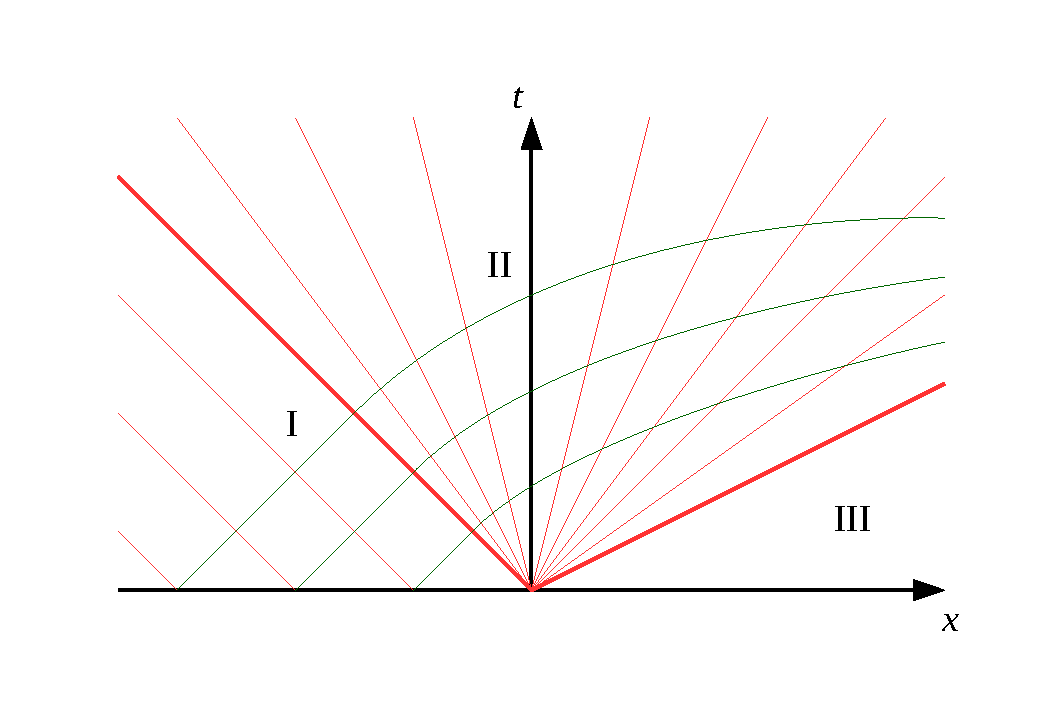
\includegraphics[width=16cm]{st-venant.pdf}
\caption{Characteristics for the St. Venant solution.}
\label{fig:st-venant-chars}
\end{center}
\end{figure}
The characteristics are sketched in Figure \ref{fig:st-venant-chars}.

In Region I, where $x < -c_0 t$, both $C_-$ and $C_+$ characteristics come from the region $x<0$ at $t=0$, and so $u=0$ and $c=c_0$. 

Assume that the $C_+$ characteristics from $x<0$ fill Region II, the region between $x=-c_0 t$ and to the left of the front. (We should check that these characteristics do in fact move faster than the front.) Then $u+2c = 2c_0$ everywhere in that region. But also $u-2c$ is constant along $C_-$ characteristics. Hence $u$ and $c$ must independently be constant along $C_-$ characteristics. Hence $C_-$ characteristics have constant slope $\lambda_- = u - c$. 

If $X_-$ is the position of a $C_-$ characteristic, then 
\begin{equation}
	\dod{X_-}{t} = u-c.
\end{equation}
So $C_-$ characteristics which start at the origin are given by
\begin{equation}
	\frac{x}{t} = u-c.
	\label{st-venant-charposition}
\end{equation}
We solve (\ref{st-venant-charposition}) together with $u+2c=2c_0$ to solve for $u$ and $c$:
\begin{align}
	u &= \frac{2}{3} \left(c_0 + \frac{x}{t}\right) \\
	c &= \frac{1}{3} \left(2c_0 - \frac{x}{t}\right) \\
	h &= \frac{1}{9g} \left(2c_0 - \frac{x}{t}\right)^2.
\end{align}
In particular, $h = 0$ at $x = 2c_0 t$, so the front moves at speed $2c_0$. On the other hand,
\begin{align}
	\lambda_+ &= u+c \\
			&= \frac{4}{3}c_0 + \frac{x}{3t} \\
\end{align}
is the speed at which the $C_+$ characteristics move.

\begin{figure}
\begin{center}
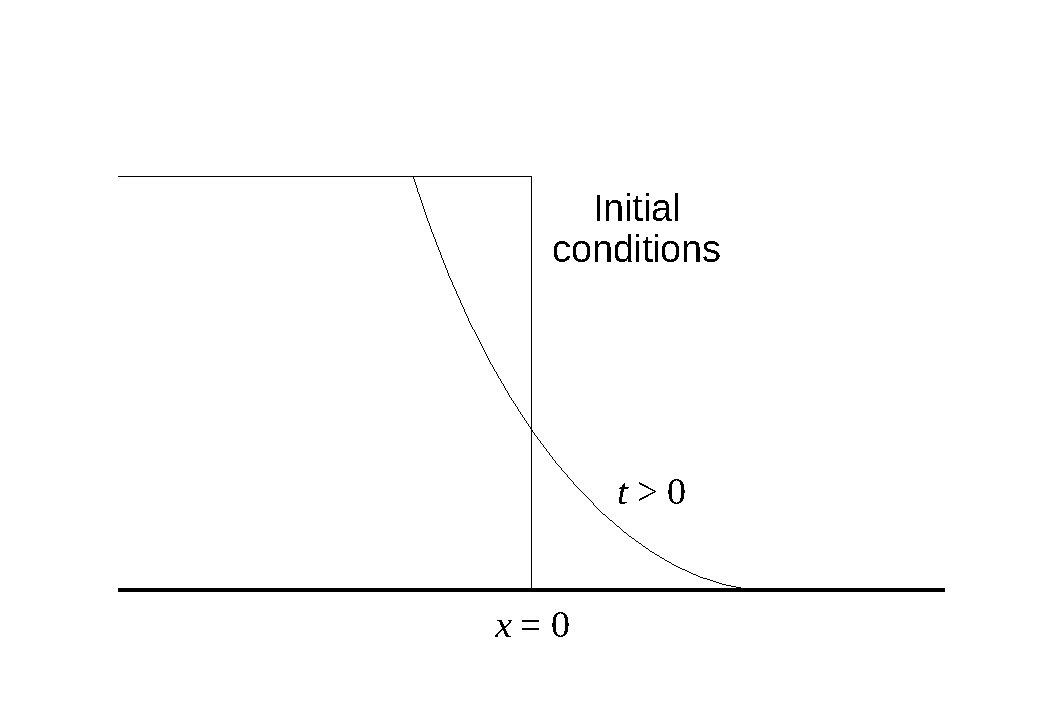
\includegraphics[width=16cm]{st-venant-solution.pdf}
\caption{The St. Venant solution.}
\label{fig:st-venant-solution}
\end{center}
\end{figure}

This is called the St. Venant solution, and it is sketched in Figure \ref{fig:st-venant-solution}. It is not observed in practice. In practice, \textit{bottom drag} and \textit{form drag} have important effects which resist motion. Bottom drag is significant if the current is much more dense than the ambient. Form drag is significant if the ambient is much more dense than the current, or if the density difference is small.

\subsubsection{Entrainment into shallow water flows}

Turbulent often produces mixing: the blending of fluid particles of a different character. If we have a turbulent shallow water flow, then not only does the turbulence transport momentum within the flow, but it can also drive mixing between the flow and the ambient fluid. In particular, if the turbulence is in the moving shallow water layer, then it can cause the layer to entrain ambient fluid into the layer, affecting its volume, density and possibly its momentum. 

This is true for \textit{miscible fluids}. Immiscible fluids can entrain each other, but the resulting two-phase flow will separate again if allowed to. 

Shallow water flows may be unstable both to short wave instabilities, such as Kelvin-Helmholtz and Holmboe instabilities, and to long wave instabilities. 

Entrainment reduces the density contrast and therefore reduces $g'$. It also increases the volume of the layer of fluid, so increases $h$. For a quiescent ambient, the result of entrainment is that $g'h$ is conserved. Also, the fluid that is being drawn in has a different (zero) momentum. 

\begin{figure}
\begin{center}
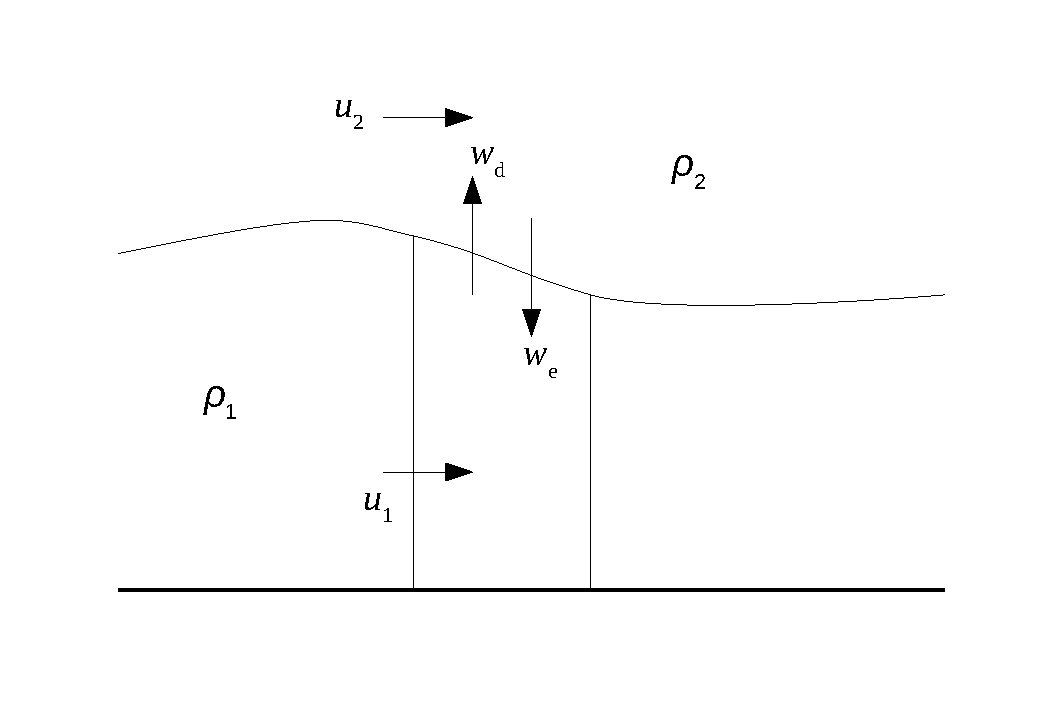
\includegraphics[width=16cm]{entrainment-shallow-water.pdf}
\caption{Schematic for entrainment/detrainment for a shallow layer.}
\label{fig:entrainment-shallow-water}
\end{center}
\end{figure}

The setup is sketched in Figure \ref{fig:entrainment-shallow-water}. Assume that the ambient fluid density $\rho_2$ is constant, so that only the density in the layer $\rho_1$ changes. Let $w_e$ be the speed of entrainment and $w_d$ the speed of `detrainment'. Then, by considering fluxes in and out of a control volume:
\begin{itemize}
	\item Conservation of volume gives
	\begin{equation}
		\dpd{h}{t} + \dpd{}{x} (u_1 h) = w_e - w_d.
	\end{equation}
	\item Conservation of mass gives
	\begin{equation}
		\dpd{}{t} (\rho_1h) + \dpd{}{x} (u_1\rho_1h) = w_e\rho_2 - w_d\rho_1
	\end{equation}
	or, using conservation of volume,
	\begin{equation}
		\dpd{\rho_1}{t} + u_1 \dpd{rho_1}{x} = -\frac{w_e}{h} (\rho_1 - \rho_2)
		\label{swentrain-mass}
	\end{equation}
	\item The momentum balance (ignoring drag) gives
	\begin{equation}
		\dpd{}{t} (\rho_1 hu_1) + \dpd{}{x}\left(
			u_1 \rho_1 hu_1 + \frac{1}{2}(\rho_1 - \rho_2)gh^2 
		\right) = w_e \rho_2 u_2 - w_d \rho_1 u_1.
	\end{equation}
	We get this by taking the pressure to be hydrostatic and equal to $p_0$ at some reference height $z_0$. Then the horizontal pressure gradient, integrated over the horizontal cross section, is 
	\begin{align}
		\int_0^h \dpd{p}{x}\dif z &= \int_0^h \dpd{}{x} (p_0 + \rho_2g(z_0-z) + (\rho_1-\rho_2)g(h-z)) \dif z \\
			&= \cdots \\
			&= \dpd{}{x} \left( \frac{1}{2}g(\rho_1-\rho_2)h^2\right).
	\end{align}
	Using conservation of mass, the momentum equation can also be written as
	\begin{equation}
		\dpd{u_1}{t} + u_1\dpd{u_1}{t} + g \frac{\rho_1-\rho_2}{\rho_1} \dpd{h}{x} + \frac{gh}{2\rho_1}\dpd{}{x}(\rho_1-\rho_2)
		 = -w_e \frac{\rho_2}{\rho_1} \frac{u_1 - u_2}{h}
		 \label{swentrain-mom}
	\end{equation}
\end{itemize}

Note that conservation of volume does not strictly hold: Mass is conserved, but the density of a mixture will be different from the density of its constituents. For `linear mixing', we can ignore changes in volume. We work in the Boussinesq approximation where $\rho_{1,2}$ are approximately equal, and assume that the ambient fluid is stationary: $u_2 = 0$. Then (\ref{swentrain-mom}) reduces to
\begin{equation}
	\dpd{u_1}{t} + u_1\dpd{u_1}{t} + g' \dpd{h}{x} + \frac{h}{2}\dpd{g'}{x}
		 = -w_e \frac{u_1}{h}
\end{equation}
where $g' = g(\rho_1-\rho_2)/\rho$. If we also write (\ref{swentrain-mass}) in terms of $g'$, then 
\begin{alignat}{5}
	\dpd{g'}{t} 		&+ u_1 \dpd{g'}{x}  		&				& 				&= -g'\frac{w_e}{h} \\
	\dpd{h}{t} 		& 					&+ u_1\dpd{h}{x}	&+ h\dpd{u_1}{x} 	&= w_e - w_d \\
	\dpd{u_1}{t} 	&+ \frac{h}{2}\dpd{g'}{x}	&+ g'\dpd{h}{x} 		&+ u_1 \dpd{u_1}{x} 	&= -u_1 \frac{w_e}{h}
\end{alignat}
or, in matrix form,
\begin{equation}
\begin{pmatrix}
 u_1 & 0 & 0 \\
 0 & u_1 & h \\
 \frac{h}{2} & g' & u_1 
\end{pmatrix}
\begin{pmatrix}
g' \\ h \\ u_1
\end{pmatrix} _x + \begin{pmatrix}g'\\h\\u_1\end{pmatrix} _t 
= 
\begin{pmatrix}
 -g'\frac{w_e}{h} \\  w_e - w_d \\  -u_1 \frac{w_e}{h}
\end{pmatrix}.
\label{swentrain-matrix}
\end{equation}

The system is still hyperbolic, as the matrix still admits three real, distinct eigenvalues: $\lambda = u_1$ and $\lambda = u_1 \pm (g'h)^{1/2}$. The latter two represent interfacial waves as before; the characteristic with $\lambda = u_1$ represents the advection of density. Since the RHS of (\ref{swentrain-matrix}) is nonzero, the evolution equations along those characteristics are inhomogeneous:
\begin{itemize}
	\item Along the $\lambda = u_1$ characteristic, we have
	\begin{equation}
		\dpd{g'}{s} = -g' \frac{w_e}/h;
	\end{equation}
	\item along the $\lambda = u_1 + (g'h)^{1/2}$ characteristic,
	\begin{equation}
		\frac{h}{2\sqrt{g'}} \dpd{g'}{s} + \sqrt{g'} \dpd{h}{s} + \sqrt{h} \dpd{u_1}{s}
		 = -\frac{1}{2}\sqrt{g'} w_e + \sqrt{g'} (w_e + w_d) - u_1 \frac{w_e}{\sqrt{h}}.
	\end{equation}
\end{itemize}


\subsection{Gravity currents}
\subsubsection{A moving dam problem}
\subsubsection{Description}
\subsubsection{Early models}
\subsubsection{Cavity flows}
\subsubsection{*Morden and Beiburg}
\subsubsection{Gravity currents and characteristics}
\subsubsection{Modelling gravity currents}
\subsubsection{Real life is more complex}


\section{Particle-laden and granular flow}

We consider the flow of a current consisting of a fluid with a well-mixed
suspension of particles, with the particles denser than the fluid. The
difference in density means that \textit{buoyancy} has a role to play. The flow is
driven by a pressure gradient and affected by the effects of buoyancy. Viscosity
is negligible, so buoyancy and inertia balance each other. 

Particles can settle out of suspension (\textit{sedimentation}) or be \textit{entrained}
into suspension. This means the concentration of the particles in the suspension
changes. So the density difference between the suspension and the ambient fluid
changes too. 

\subsection{Types of particulate flows}

We model four types of particulate gravity currents. The models are ad-hoc and
apply to different geophysical situations, where different assumptions may be
made about the flows and the particles:

\paragraph{Grain suspension by fluid turbulence} Examples include pyroclastic
flows
%\footnote{Wikipedia: A pyroclastic flow is a fast-moving current of hot gas and
%rock (collectively known as tephra), which reaches speeds moving away from a
%volcano of up to 700 km/h (450 mph). The gas can reach temperatures of about
%1,000\deg C. Pyroclastic flows normally hug the ground and travel downhill, or
%spread laterally under gravity. Their speed depends upon the density of the
%current, the volcanic output rate, and the gradient of the slope. They are a
%common and devastating result of certain explosive volcanic eruptions.}
, turbidity currents
\footnote{Wikipedia: A turbidity current is a current of rapidly moving,
sediment-laden water moving down a slope through water, or another fluid. The
current moves because it has a higher density than the fluid through which it
flows—the driving force of a turbidity current derives from its sediment, which
renders the turbid water denser than the clear water above. The deposit of a
turbidity current is called a turbidite.}
and powder snow
\footnote{Wikipedia: Freshly fallen, uncompacted snow. The density and moisture
content of powder snow can vary widely; snowfall in coastal regions and areas
with higher humidity is usually heavier than a similar depth of snowfall in an
arid or continental region. Light, dry (low moisture content, typically 4–7\%
water content) powder snow is prized by skiers and snowboarders. It is often
found in the Rocky Mountains of North America and in most regions in Japan.}. 
In such flows, the particles may be very concentrated and denser than the fluid, but
they are kept in suspension by the turbulent flow of the fluid; any particles
which settle quickly undergo \textit{resuspension}.

\paragraph{Liquefied and fluidised flow} Examples include dense snow avalanches
and \textit{some} mudflows. In these cases, the flow is dominant and the
particles move with the flow; in this regime, particles do not interact with
each other (\textit{cohesionlessness}), as they are separated from each other
(\textit{grain dispersion})). Their effect is to increase the viscosity of the
fluid. However, this limits the possibility of turbulence, and so particles can 
settle out at the base of the fluid.

\paragraph{Dry grain flow and interactions} Examples include sand dune
avalanches and rock slides. Now the particles interact with each other,
colliding fequently; the fluid acts as a lubricant. 

\paragraph{Grain-supported matrix} Examples include debris flows and lahars, or
large boulders suspended in a muddy matrix. Now cohesion has a large r\^ole to
play. The flow of mud and slurries are non-Newtonian. Effects of cohesion,
friction, pore pressure, etc. may be modelled using other stress-shear rate
relationships (\textit{rheological models}), including power laws, Bingham
plastic models nad Herschel-Bulkley models. In the latter two models, the fluid
has a \textit{yield strength}: a minimum shear stress must be applied before any
flow occurs. 

\subsection{Modelling a particulate gravity current}



\subsection{Physics within a particle gravity current}

A particle gravity current can be modelled as having a main body and a base. In
the main body, there is a well-mixed suspension of particles in a turbulent
flow; in the base, the particles and fluid have low velocity and particles are
settling out. 

Let
\begin{itemize}
 \item $\rho_0$ denote the density of the fluid;
 \item $\mu_0$ denote the viscosity of the fluid;
 \item $\rho_p$ denote the density of the particles;
 \item $\phi$ denote the concentration of particles.
\end{itemize}
Then the \textit{bulk density} of the fluid-particle mixture is
\begin{equation}
    \rho_l = \rho_0 + \phi (\rho_p - \rho_0) 
\end{equation}
and the \textit{reduced gravity} is
\begin{equation}
 g' = g \frac{\rho_l - \rho_0}{\rho_0} = \phi g \frac{\rho_p - \rho_0}{\rho_0} = \phi g_0'
\end{equation}
where
\begin{equation}
    g_0' = g \frac{\rho_p - \rho_0}{\rho_0}.
\end{equation}

\subsection{Sedimenting particle-laden flows}

We now assume that particles are small compared to the scale of motion, so that
the presence of an individual particle has a negligible effect on the bulk flow.
However, the collective of particles will have an effect. We also assume that
particles sediment slowly, over a timescale much larger than that of the flow;
and that particles are numerous and well-mixed, so that we can talk of the
`concentration' of particles, rather than having to study individual particles.

Although we use the word `particles', this theory could just as well apply to
bubbles or to droplets; a bubble can be regarded as a particle with density
negligible compared to that of the fluid; the reduced gravity is negative.

The suspension changes the bulk properties of the fluid. As discussed, the 
suspension has density
\begin{equation}
        \rho_l = \rho_0 + \phi (\rho_p - \rho_0).
\end{equation}
The viscosity of the suspension is given by a power law
\begin{equation}
 \mu = \mu_0 \left( 1 - \frac{\phi}{\phi_{max}} \right)^{-n \phi_{max}}
\end{equation}
where $\phi_{max}$ is the maximum suspension concentration that can be
supported. For spherical particles, $n = \frac{5}{2}$.

Particles settle towards the bottom at some settling velocity $u_s$ which we
will determine. Let $D$ denote the particle diameter. We define the
\textit{particle Reynolds number}
\begin{equation}
    Re_p = \frac{\rho_l D u_s}{\mu}
\end{equation}
which governs many properties of the flow.

When particles sediment out of suspension, we are left with a \textit{clarified}
fluid, devoid of particles, and a concentrated suspension at the bottom where
all the particles gather. Sedimenting flows are classified into four types:
\begin{itemize}
    \item Type I: Free settling of individual particles
    \item Type II: Flocculant settling: Coaleescence of particles
    \item Type III: Hindered (zone) settling: Restricted, fluid motion
    \item Type IV: Compression settling: Mechanical support
\end{itemize}
We will discuss Types I and III in detail.

\subsubsection{Type I: Free settling of individual particles} 

This occurs when particles are very well-separated from each other, and may be
treated independently of each other.

\paragraph{The particle Reynolds number} When a sphere of diameter $D$ moves at
a speed $u_s$ through otherwise unmoving fluid, its behaviour depends on the
particle Reynolds number $Re_p=\frac{\rho_lDu_s}{\mu}$.  If $Re_p\ll 1$ then the
flow past the sphere is \textit{laminar}; the sphere travels smoothly. But if
$10^3 \ll Re_p \ll 2\cdot10^5$ then the flow is in the \textit{inertial regime};
the sphere travels roughly, and the boundary layer is turbulent. 

Various other regimes are possible for different values of $Re_p$; they are
discussed in Middleton and Southard (1984). 

\paragraph{The drag coefficient} By dimensional analysis, the drag $F_D$ on a
particle travelling at $u_s$ through a fluid must be proportional to
$\frac{1}{2}\rho_lu_s^2A_p$:
\begin{equation}
 F_D = C_D\frac{1}{2}\rho_lu_s^2A_p
\end{equation}
where $A_p$ is the planar area of the particle. (See Prandtl and Tietjens, 1957
for details.) The dimensionless coefficient $C_D$ is called the \textit{drag
coefficient}, and depends on the Reynolds number. The dependence may be found
empirically:
\begin{itemize}
 \item When $Re_p\ll1$, then $C_D$ is inversely proportional to $Re_p$:
\begin{equation}
    C_D = \frac{24}{Re_p}
\end{equation}
 \item When $0.2 < Re_p < 10^3$, there is a transitional region.
 \item When $10^3 < Re_p < 2\cdot10^5$, $C_D$ is approximately constant for
     cylinders, spheres and discs. For these shapes, $C_D \approx 0.44$.
 \item At $Re_p\approx2\cdot10^5$, the drag coefficient drops very quickly before
     increasing much more slowly again. This is called the \textit{drag crisis
     regime}, and arises because of a flow separation.
\end{itemize}

\paragraph{The settling velocity} So what is the settling velocity $u_s$?
We consider the momentum balance on a particle in suspension. The forces acting
on the particle are drag, buoyancy and gravity, and so:
\begin{align}
    m\frac{du}{dt} &= F_g - F_b - F_D \\
    F_D            &= C_D\frac{1}{2}\rho_lu^2A_p \\
    F_b            &= \rho_lgV \\
    F_g            &= \rho_pgV
\end{align}
where $V$ is the volume of the particle. The expression for $F_b$ is given by
Archimedes' law: the buoyancy force is $g$ times the mass of fluid displaced.
(Note that the fluid displaced is assumed to have density $\rho_l$ rather than
$\rho_0$, even though we are assuming that particles are well-separated from
each other and do not interact!) Setting $\frac{du}{dt} = 0$ and solving for $u$
gives us the terminal velocity, which is the settling velocity.

For a sphere of diameter $D$, we have $V = \frac{1}{6}\pi D^3$ and $A_p =
\frac{1}{4}\pi D^2$, and so
\begin{equation}
    u_s=\sqrt{\frac{4g(\rho_p-\rho_l)D}{3C_D\rho_l}}.
\end{equation}
Recall that in the Stokes regime $Re_p < 0.2$, we have $C_D=\frac{24}{Re_p}$. Hence:
\begin{align}
    F_D &= 3\pi u_s \mu D \\
    u_s &= \frac{g(\rho_p-\rho_l)D^2}{18\mu}
\end{align}
with $u_s \propto D^2$ and dependent on $\mu$. 

But in the inertial, turbulent regime, with $10^3 < Re_p < 2\cdot10^5$, we have
that $C_D=0.44$ is constant, and 
\begin{align}
    F_D &= 0.055\pi\rho_lu_s^2D^2 \\
    u_s &= 1.74\sqrt{\frac{g(\rho_p-\rho_l)D}{\rho_l}}
\end{align}
with $u_s \propto D^{1/2}$ and not dependent on $\mu$.

These predictions are confirmed by observations: the Stokes regime holds for
fine grains such as silt, whereas the inertial regime holds for very coarse
sand, granules and pebbles (provided that particle-particle interactions may be
neglected). However, for $D$ between 0.1mm and 1mm (such as for medium or coarse
sand), neither the Stokes nor the turbulent predictions hold well. Many
equations have been proposed to describe the intermediate region, including the
\textit{Ferguson-Church equation}.  \footnote{See
\url{http://hinderedsettling.com/2013/08/09/grain-settling-python/}.}

\paragraph{Advection and diffusion of particles} The concentration of particles
$\phi$ is governed by an advection-diffusion equation:
\begin{equation}
    \frac{\partial\phi}{\partial t} + \mathbf{u}\cdot\nabla\phi = D\nabla^2\phi
\end{equation}
where $D$ now denotes a diffusion coefficient, \textit{not} the particle
diameter. The particle velocity $\mathbf{u}$ is equal to the velocity of the
fluid, plus the settling velocity:
\begin{equation}
    \mathbf{u} = (u, v, w) + (0, 0, -u_s).
\end{equation}
In the particular case of no background fluid flow, $\mathbf{u} = (u,v,w)$ and
the advection-diffusion equation reduces to
\begin{equation}
    \frac{\partial\phi}{\partial t} - u_s\frac{\partial\phi}{\partial z} = D\nabla^2\phi
\end{equation}

The diffusion coefficient $D$ depends on $Re_p$ and whether the flow is laminar
or turbulent. In the laminar regime, diffusion of particles is due to molecular
(Brownian) diffusion: 
\begin{equation}
    D = D_B \sim \frac{kT}{6\pi\mu r}
\end{equation}
where $r$ is the radius of particles, $k$ is the Boltzmann constant and $T$ is
the temperature. Molecular diffusion is a very slow process unless $r$ is very
small, such as for aerosol particles.

However, in the turbulent regime, diffusion of particles is due to turbulent
diffusivity:
\begin{equation}
    D = D_t \sim u^\star h
\end{equation}
where $u^\star = \sqrt{\frac{\tau_b}{\rho}}$ is the shear velocity (friction
velocity), $\tau_b$ is the shear stress at the bottom, and $h$ is some length
scale, such as the distance from the bottom.

\subsubsection{Type III: Hindered (zone) settling}

When there are many particles, then particles no longer settle at $u_s$ but at
some slower velocity, $u_h$, which depends on $\phi$ and on $u_s$. 




%\newpage
\chapter{Buoyancy-driven flows} \label{section-woods}

In these lectures we will consider flows which are turbulent, driven by
buoyancy, and possibly containing several phases, such as suspensions of ash in
air.  Turbulence is important because it is ubiquitous, and is responsible for
mixing.

Jets, plumes and fountains are three different types of such things.

We will try to model phenomena such as volcanic plumes, which rise turbulently
for twenty or thirty kilometres. A volcanic plume is able to rise so high
because it starts off with plenty of thermal energy, not just kinetic energy (as
for a jet). 




\newpage
\chapter{Particle-laden and granular flow} \label{section-nmv}

\section{Types of particulate flows}

Models for particulate flows are ad-hoc and apply to different geophysical situations, depending on which assumptions may be made about the flows and the particles:

\paragraph{Grain suspension by fluid turbulence} Examples include pyroclastic
flows\footnote{Wikipedia: A pyroclastic flow is a fast-moving current of hot gas
    and rock (collectively known as tephra), which reaches speeds moving away
    from a volcano of up to 700 km/h (450 mph). The gas can reach temperatures
    of about $1,000\,^{\circ}\mathrm{C}$. Pyroclastic flows normally hug the
    ground and travel downhill, or spread laterally under gravity. Their speed
    depends upon the density of the current, the volcanic output rate, and the
    gradient of the slope. They are a common and devastating result of certain
explosive volcanic eruptions.}, turbidity currents\footnote{Wikipedia: A
    turbidity current is a current of rapidly moving, sediment-laden water
    moving down a slope through water, or another fluid. The current moves
    because it has a higher density than the fluid through which it flows—the
    driving force of a turbidity current derives from its sediment, which
    renders the turbid water denser than the clear water above. The deposit of a
turbidity current is called a turbidite.} and powder snow\footnote{Wikipedia:
    Freshly fallen, uncompacted snow. The density and moisture content of powder
    snow can vary widely; snowfall in coastal regions and areas with higher
    humidity is usually heavier than a similar depth of snowfall in an arid or
    continental region. Light, dry (low moisture content, typically 4–7\% water
    content) powder snow is prized by skiers and snowboarders. It is often found
in the Rocky Mountains of North America and in most regions in Japan.}. In such
flows, the particles may be very concentrated and denser than the fluid, but
they are kept in suspension by the turbulent flow of the fluid; any particles
which settle quickly undergo \textit{resuspension}.

\paragraph{Liquefied and fluidised flow} Examples include dense snow avalanches
and \textit{some} mudflows. In these cases, the flow is dominant and the
particles move with the flow; in this regime, particles do not interact with
each other (\textit{cohesionlessness}), as they are separated from each other
(\textit{grain dispersion}). Their effect is to increase the viscosity of the
fluid. However, this limits the possibility of turbulence, and so particles can 
settle out at the base of the fluid.

\paragraph{Dry grain flow and interactions} Examples include sand dune
avalanches and rock slides. Now the particles interact with each other,
colliding fequently; the fluid acts as a lubricant. 

\paragraph{Grain-supported matrix} Examples include debris flows and lahars, or
large boulders suspended in a muddy matrix. Now cohesion has a large r\^ole to
play. The flow of mud and slurries are non-Newtonian. Effects of cohesion,
friction, pore pressure, etc. may be modelled using other stress-shear rate
relationships (\textit{rheological models}), including power laws, Bingham
plastic models nad Herschel-Bulkley models. In the latter two models, the fluid
has a \textit{yield strength}: a minimum shear stress must be applied before any
flow occurs. 

\section{Physics within a particle gravity current}

A particle gravity current can be modelled as having a main body and a base. In
the main body, there is a well-mixed suspension of particles in a turbulent
flow; in the base, the particles and fluid have low velocity and particles are
settling out. 

We consider the flow of a current consisting of a fluid with a well-mixed
suspension of particles, with the particles denser than the fluid. The
difference in density means that \textit{buoyancy} has a role to play. The flow
is driven by a pressure gradient and affected by the effects of buoyancy.
Viscosity is negligible, so buoyancy and inertia balance each other. 

Particles can settle out of suspension (\textit{sedimentation}) or be
\textit{entrained} into suspension. This means the concentration of the
particles in the suspension changes. So the density difference between the
suspension and the ambient fluid changes too. 

Let
\begin{itemize}
 \item $\rho_0$ denote the density of the fluid;
 \item $\mu_0$ denote the viscosity of the fluid;
 \item $\rho_p$ denote the density of the particles;
 \item $\phi$ denote the concentration of particles.
\end{itemize}
Then the \textit{bulk density} of the fluid-particle mixture is
\begin{equation}
    \rho_l = \rho_0 + \phi (\rho_p - \rho_0) 
\end{equation}
and the \textit{reduced gravity} is
\begin{equation}
 g' = g \frac{\rho_l - \rho_0}{\rho_0} = \phi g \frac{\rho_p - \rho_0}{\rho_0} = \phi g_0'
\end{equation}
where
\begin{equation}
    g_0' = g \frac{\rho_p - \rho_0}{\rho_0}.
\end{equation}

\section{Sedimenting particle-laden flows}

We assume that particles are small compared to the scale of motion, so that the presence of an individual particle has a negligible effect on the bulk flow. However, the collective of particles will have an effect. We also assume that particles sediment slowly, over a timescale much larger than that of the flow; and that particles are numerous and well-mixed, so that we can talk of the `concentration' of particles, rather than having to study individual particles.

Note that although we use the word `particles', all of this theory could just as well apply to bubbles or to droplets; a bubble can be regarded as a particle with density negligible compared to that of the fluid; the reduced gravity is negative.

The suspension changes the bulk properties of the fluid. As discussed, the suspension has density
\begin{equation}
        \rho_l = \rho_0 + \phi (\rho_p - \rho_0)
\end{equation}
where $\phi$ is the concentration by volume. We model the viscosity of the suspension as having a power law dependence on the concentration: 
\begin{equation}
 \mu = \mu_0 \left( 1 - \frac{\phi}{\phi_{max}} \right)^{-n \phi_{max}}
\end{equation}
where $\phi_{max}$ is the maximum suspension concentration that can be supported. For spherical particles, $n = \frac{5}{2}$.
\footnote{A similar result is derived in a \textit{Slow Viscous Flow} past examination question, 2013/68/1.}

We define the \textit{particle Reynolds number}
\begin{equation}
    \mathrm{Re}_p = \frac{\rho_l D u_s}{\mu}
\end{equation}
which governs many properties of the flow. Here $D$ is the diameter of a particle, and $u_s$ is the settling velocity, which we will determine. 

When particles sediment out of suspension, we are left with a \textit{clarified} fluid, devoid of particles, and a concentrated suspension at the bottom where all the particles gather. 

Sedimenting flows can exhibit four types of behaviour, depending on $\mathrm{Re}_p$ and on the concentration $\phi$:
\begin{itemize}
    \item Type I: Free settling of individual particles
    \item Type II: Flocculant settling: Coaleescence of particles
    \item Type III: Hindered (zone) settling: Restricted, fluid motion
    \item Type IV: Compression settling: Mechanical support
\end{itemize}
We will discuss Types I and III in detail. Types II and IV involve complicated particle-particle interactions. 

\subsection{Type I: Free settling of individual particles} 

This occurs when particles are very well-separated from each other, and so do not interact with each other. This occurs at very low concentrations (the \textit{dilute limit}).

\paragraph{The particle Reynolds number} When a sphere of diameter $D$ moves at a speed $u_s$ through otherwise unmoving fluid, its behaviour depends on the particle Reynolds number $\mathrm{Re}_p=\frac{\rho_lDu_s}{\mu}$.  If $\mathrm{Re}_p\ll1$ then the flow past the sphere is \textit{laminar}; the sphere travels smoothly. But if $10^3 \ll \mathrm{Re}_p \ll 2\cdot10^5$ then the flow is in the \textit{inertial regime}; the sphere travels roughly, and the boundary layer on the sphere is turbulent. Various other regimes are possible for different values of $\mathrm{Re}_p$; they are discussed in Middleton and Southard (1984). 

\paragraph{The drag coefficient} By dimensional analysis, the drag $F_D$ on a particle travelling at $u_s$ through a fluid is
\begin{equation}
 F_D = C_D\frac{1}{2}\rho_lu_s^2A_p
\end{equation}
where $A_p$ is the planar area of the particle. (See Prandtl and Tietjens, 1957 for details.) The dimensionless coefficient $C_D$ is called the \textit{drag coefficient}, and depends on the Reynolds number. The dependence may be found empirically:
\begin{itemize}
	\item When $\mathrm{Re}_p\ll1$, then $C_D$ is inversely proportional to $\mathrm{Re}_p$:
	\begin{equation}
    		C_D = \frac{24}{\mathrm{Re}_p}
	\end{equation}
	\item When $0.2 < \mathrm{Re}_p < 10^3$, there is a transitional region.
	\item When $10^3 < \mathrm{Re}_p < 2\cdot10^5$, $C_D$ is approximately constant for cylinders, spheres and discs. For these shapes, $C_D \approx 0.44$.
	\item At $\mathrm{Re}_p\approx2\cdot10^5$, the drag coefficient drops very quickly before increasing much more slowly again. This is called the \textit{drag crisis regime}, and arises because of a flow separation.
\end{itemize}

\paragraph{The settling velocity} So what is the settling velocity $u_s$? We consider the momentum balance on a particle in suspension. The forces acting on the particle are drag, buoyancy and gravity, and so:
\begin{align}
    m\dod{u}{t} &= F_g - F_b - F_D \\
    F_D            &= C_D\frac{1}{2}\rho_lu^2A_p \\
    F_b            &= \rho_lgV \\
    F_g            &= \rho_pgV
\end{align}
where $V$ is the volume of the particle. The expression for $F_b$ is given by Archimedes' law: the buoyancy force is $g$ times the mass of fluid displaced. (Note that the fluid displaced is said to have density $\rho_l$ rather than $\rho_0$, though the two are approximately equal in the dilute limit.) Setting $\od{u}{t} = 0$ and solving for $u$ gives us the terminal velocity, which is the settling velocity.

For a sphere of diameter $D$, we have $V = \frac{1}{6}\pi D^3$ and $A_p = \frac{1}{4}\pi D^2$, and so
\begin{equation}
    u_s=\sqrt{\frac{4g(\rho_p-\rho_l)D}{3C_D\rho_l}}.
\end{equation}
Recall that in the Stokes regime with $\mathrm{Re}_p < 0.2$, we have $C_D=\frac{24}{\mathrm{Re}_p}$. Hence:
\begin{align}
    F_D &= 3\pi u_s \mu D \\
    u_s &= \frac{g(\rho_p-\rho_l)D^2}{18\mu}
\end{align}
with $u_s \propto D^2$ and dependent on $\mu$. But in the inertial, turbulent regime, with $10^3 < \mathrm{Re}_p < 2\cdot10^5$, we have $C_D=0.44$ constant, and 
\begin{align}
    F_D &= 0.055\pi\rho_lu_s^2D^2 \\
    u_s &= 1.74\sqrt{\frac{g(\rho_p-\rho_l)D}{\rho_l}}
\end{align}
with $u_s \propto D^{1/2}$ and not dependent on $\mu$.

These predictions are confirmed by observations: the Stokes regime holds for fine grains such as silt, whereas the inertial regime holds for very coarse sand, granules and pebbles (provided that particle-particle interactions may be neglected). However, for $D$ between 0.1mm and 1mm (such as for medium or coarse sand), we are in the transitional regime where neither the Stokes nor the turbulent predictions hold well. Many equations have been proposed to describe the intermediate region, including the \textit{Ferguson-Church equation}.\footnote{See \url{http://hinderedsettling.com/2013/08/09/grain-settling-python/}.}

\paragraph{Advection and diffusion of particles} The concentration of particles $\phi$ is governed by an advection-diffusion equation:
\begin{equation}
	\dpd{\phi}{t} + \bs{u}\cdot\grad\phi = D\grad^2\phi
	\label{suspension-advdiff}
\end{equation}
where $D$ now denotes the diffusion coefficient, \textit{not} the particle diameter. The settling velocity which we have so far calculated was for an otherwise stationary fluid, so in (\ref{suspension-advdiff}) the particle velocity $\bs{u}$ is equal to
\begin{equation}
 	\mathbf{u} = (u, v, w) + (0, 0, -u_s)
\end{equation}
where $(u,v,w)$ is the mean velocity of the fluid.\footnote{We can have fluid flow even if there is no mean fluid flow, if we are in a turbulent regime.}

If there is no mean background fluid flow, then (\ref{suspension-advdiff}) reduces to
\begin{equation}
    \dpd{\phi}{t} - u_s\dpd{\phi}{z} = D\grad^2\phi.
    \label{suspension-advdiff-settling}
\end{equation}
If we neglect dependencies on $x$ and $y$, then (\ref{suspension-advdiff-settling}) is Burgers' equation. 

The diffusion coefficient $D$ depends on $\mathrm{Re}_p$ and whether the flow is laminar or turbulent. In the laminar regime, diffusion of particles is due to molecular (Brownian) diffusion: 
\begin{equation}
    D = D_B \sim \frac{kT}{6\pi\mu r}
\end{equation}
where $r$ is the radius of particles, $k$ is the Boltzmann constant and $T$ is the temperature. Molecular diffusion is a very slow process unless $r$ is very small, such as for aerosol particles.

However, in the turbulent regime, diffusion of particles is due to turbulent diffusivity:
\begin{equation}
    D = D_T \sim u^\star h
\end{equation}
where $u^\star = \sqrt{\frac{\tau_b}{\rho}}$ is the shear velocity (friction velocity), $\tau_b$ is the shear stress at the bottom, and $h$ is some turbulence length scale, such as the distance from the bottom.

Note that if we ignore diffusivity in Equation \ref{suspension-advdiff-settling} and set $D=0$, then the resulting equation admits shocks. This is because when the diffusivity is small, we have fronts where the concentration changes very sharply. To calculate the speed at which these fronts move, we can use the Rankine-Hugoniot conditions.

\subsection{Type II: Flocculent settling, particle coalescence}

In this regime, particles may coalesce together to form larger particles, which have larger settling velocities. Therefore settling in this regime occurs quicker than if particles do not coalesce. There is no mathematical theory to model this regime.

\subsection{Type III: Hindered (zone) settling}

When there are many particles, then particles no longer settle at the $u_s$ which we have calculated, but at some slower velocity $u_h$, a \textit{hindered settling velocity}. The hindered settling velocity depends on $\phi$ and on $u_s$. As $\phi$ increases, $u_h$ decreases. As $\phi$ approaches $\phi_{max}$, then more complicated inter-particle interactions take place and we start to have compression settling. 

The model that we will use is 
\begin{equation}
	u_h = u_s \left( 1 - \frac{\phi}{\phi_max} \right)^\alpha
\end{equation}
where $\alpha$ is some empirically determined constant which depends on the flow regime.\footnote{Following 'A physical introduction to suspension dynamics'.} Richardson and Zaki (1954) found that for $\phi$ up to 0.35, $\alpha = 4.65$ in the laminar regime $\mathrm{Re}_p < 0.2$ and $\alpha = 2.39$ in the regime $\mathrm{Re}_p > 500$. 
%TODO proper citations

The settling flux is
\begin{equation}
	Q_h = u_h \phi.
\end{equation}
In a suspension with a steady concentration profile $\phi(z)$, the settling flux of particles downwards is balanced by diffusive flux upwards. Thus the concentration satisfies the \textit{Rouse equation}:
\begin{equation}
	\phi(z) u_h(z) = -D \dod{\phi(z)}{z}
\end{equation}
where $D$ is a diffusivity. This tends to happen if the flow is turbulent and $D$ is large.

\paragraph{Nonlinear kinematic wave equation}
If $\phi = \phi(z,t)$ and diffusivity is small (which happens if the flow is laminar) then, as we have seen before, $\phi$ obeys the `traffic equation'
\begin{equation}
	\dpd{\phi}{t} + \dpd{\phi u_h}{z} = 0
\end{equation}
which may be solved by the method of characteristics. Again, solutions to this equation have shocks, which represent sharp fronts in a settling suspension.

\paragraph{Settling of particles on inclines}

\subsection{Type IV: Compressional settling, compacting}

This regime occurs in regions of very high concentration. Stirring or tapping can allow the liquid to escape. The packing fraction may increase locally, leading to increased stability.  
%TODO

\section{Modelling a particulate gravity current}

See \cite{huppert-1998} for more details and more complicated models.

\subsection{A simple box model}
We assume a `box profile' for the particulate gravity current: it has a length
$L(t)$ and a constant height $h(t)$ throughout its length, except possibly at
its nose, where the nose height $h_N$ may be larger than $h$. We let $u$ be the
velocity in the current, and $u_N$ be the velocity of the nose. The nose
velocity is related to $L$ by $\od{L}{t} = u_N$. For simplicity we will take
$h_N = h$ and $u_N = u$. We will also assume that the particle concentration
$\phi$ is uniform throughout the current, and that particles are settling with
settling velocity $u_s$.  

Throughout, we assume that $\phi\ll1$, so that the settling is unhindered, and the current is Boussinesq. 

Let $\rho_0$ be the fluid density, and $\rho_p$ be the particle density. Then the density of the current, with concentration $\phi$, is $\rho_l = (1-\phi)\rho_0 + \phi \rho_p$. We define a reduced gravity
\begin{equation}
g' = g \frac{\rho_l - \rho_0}{\rho_0} = g\phi\frac{\phi_p - \phi_0}{\rho_0} = \phi g'_0.
\end{equation} 
Since the current is Boussinesq, $g' \ll g$. 

Assume that there is no entrainment. Then the volume of the current is constant, and so the mass of the current $M = L(t)h(t)$ is constant. Hence particle conservation gives
\begin{equation}
\dod{(M\phi)}{t} = M\dod{\phi}{t} = -u_s \phi(t) L(t)
\end{equation}
Hence,
\begin{equation}
\dod{\phi}{t} = -\frac{u_s \phi}{h}.
\end{equation}

Meanwhile, the value of $u_N = \od{L}{t}$ is related to the nose height $h_N$ by a Froude number condition
\begin{equation}
u_N = \dod{L}{t} = \mathrm{Fr}_f (\phi g_0' h_N)^{1/2} 
 \label{pcbox-dLdt}
\end{equation}
where $\mathrm{Fr}_f$ is the front Froude number. For an ideal fluid with
irrotational flow, Bernoulli's theorem would predict that $\mathrm{Fr}_f =
\sqrt{2}$, but in practice experiments by Huppert \textit{et al.} have shown
that $\mathrm{Fr}_f = 1.19$ for particulate gravity currents.\cite{huppert-1998}

Assume that $h_N = h$ and $u_N = u$. We must solve these equations for $\phi$ and $L$, subject to some initial conditions $L=L_0$ and $\phi=\phi_0$ at $t=0$. One way to proceed would be to eliminate one of $\phi$ or $L$, and get the equation
\begin{equation}
 \dod{}{t}\left[ L\left( \dod{L}{t}\right)^2 \right] = -\frac{u_s L}{h} \left(\dod{L}{t}\right)^2
\end{equation}
which must be solved numerically. We can also make progress by dividing one equation by the other, to get
\begin{equation}
\dod{\phi}{L} = -\frac{u_s L}{h} \frac{1}{\mathrm{Fr}_f (\phi g_0' h)^{1/2}} = -\frac{\phi^{1/2} L^{3/2}}{\beta} 
 \label{pcbox-dphidL}
\end{equation}
where
\begin{equation}
\beta = \frac{\mathrm{Fr}_f (g_0' M^3)^{1/2}}{u_s}
\end{equation}

Equation \ref{pcbox-dphidL} can be solved easily:
\begin{equation}
 L^{5/2} =  L_0^{5/2} + 5\beta \left(\phi_0^{1/2} - \phi^{1/2} \right) 
 \label{pcbox-Lphi}
\end{equation}
The current stops advancing when the concentration drops to $\phi = 0$. Hence the run-out length of the current $L_\infty$ is
\begin{equation}
 L_\infty^{5/2} =  L_0^{5/2} + 5\beta \phi_0^{1/2}.
\end{equation}
We can therefore rearrange (\ref{pcbox-Lphi}):
\begin{equation}
 \frac{\phi}{\phi_0} = \left[ 1-\left(\frac{L}{L_\infty}\right)^{5/2} \right]^2 = \left[ 1 - \xi^{5/2} \right]^2
\end{equation}
where $\xi = L/L_\infty$. 
Having found $\phi$ in terms of $L$ and $L_\infty$, we can solve (\ref{pcbox-dLdt}) implicitly for $t$ as a function of $L$. 

\section{Sediment transport}

Particles in a fluid can move by several means. Particles which are in
suspension (the \textit{suspended load}) or which have dissolved (the
\textit{dissolved load}) will move with the flow. Particles which have settled
to the bottom of the fluid can roll or slide along the bottom, or by hopping
(\textit{saltation}). In a river, silt and clay tend to move by suspension; sand
particles, which are larger, by saltation; gravel, larger still, by rolling and
sliding. 

A particle out of suspension does not necessarily move when there is a flow. A
rock on the bed starts to move only when the flow exerts a critical shear stress
on the bed. However, if the flow is turbulent then a sudden eddy may be able to
move the rock: turbulent flows are stochastic, and need to be modelled as such. 

Transport will change the morphology of the bed by erosion deposition: a strong
flow can break up large rocks into smaller pieces. This in turn changes whether
these particles are able to be suspended or settle out of suspension.  

\subsection{Resuspension}

Resuspension is the process by which particles which have settled to the bottom
boundary are lifted back up into suspension in the fluid. A flow near a boundary
obeys the no-slip condition at the boundary, but away from the boundary suppose
the velocity is uniform, horizontal, with speed $U$. There is a viscous sublayer
of thickness $\delta\sim\nu/U$ near the boundary, where the speed drops from $U$
to $0$. The velocity profile in the viscous sublayer is approximately linear.
The shear stress on the boundary is $O(\mu U/\delta) = O(\rho U^2)$.

Consider a particle deposited in the viscous sublayer. Since the fluid at the
top of the particle moves faster than the fluid at the bottom, then by
Bernoulli's principle the pressure at the bottom of the particle is higher than
the pressure at the top. This causes \textit{lift}. If the particle is more
dense than the fluid, then it also experiences a `downwards' \textit{buoyancy}
force. 

\section{Aqueous and aeolian bedforms (dunes)}

\section{Dry granular flows, rheology, segregation}

Granular materials do not fill the space that they occupy, but instead have a
\textit{packing fraction} $\phi$. The packing fraction is variable for a given
material: a collection of uniform rigid spheres has a maximum packing fraction
of $\phi\approx0.74$, but randomly packed spheres have typically
$\phi\approx0.64$. The value of the packing fraction depends on the history of
the material: that is, how it came to be arranged as it is. A pile of sand could
have very different packing fractions depending on whether the sand was simply
poured onto a surface, or slowly added and packed together. 

Like a viscous fluid, a granular flow on a inclined plane or chute executes a
shear flow $u = U(z)$. But unlike a viscous fluid, the cross-depth velocity
profile $U$ is not quadratic in $z$, and the shear stress $\tau_{xz}$ is not linearly
proportional to the shear rate $\dot\gamma = U'(z)$. Bagnold (1954) showed by
simple collisional arguments and through experiments that, for spherical grains,
$\tau_{xz}$ is in fact proportional to $\dot\gamma^2$.\cite{bagnold-1954}
\footnote{Bagnold's experiments were conducted with a suspension of grains in a
viscous fluid. At high shear rates, the viscosity of the fluid could be
neglected, compared to the inertia of the grains, and $\tau_{xz}\propto\dot\gamma^2$.
At low shear rates, this simply behaves as a particle-laden viscous flow;
$\tau_{xz}\propto\dot\gamma$ but with a higher effective viscosity as discussed
above.}
This stress-strain relation would give rise to what is called the
\textit{Bagnold velocity profile}.

Bagnold (1954) also showed that the grains also exert a normal stress
$\tau_{zz}$ on each other, owing to their collitions; this serves to 

The Bagnold relation $\tau_{xz} \propto\dot\gamma^2$ was derived for this
particular geometry. There have been subsequent attempts to find more general
constitutive relations for dense granular flows. This study is called
\textit{rheology}. A recently-developed theory is that of Jop \textit{et al.}
(2006), the $\mu(I)$ rheology. In the $\mu(I)$ rheology, the shear stress $T$ is
taken to be equal to $\mu(I) P$, where $P$ is the pressure (normal stress). The
coefficient of friction $\mu$ is taken to be a function of the \textit{inertial
number} $I = \dot\gamma d (P / \rho_s)^{1/2}$, a nondimensionalised shear
rate.\cite{jop-2006}

A granular flow with particles of different sizes or densities will exhibit
\textit{segregation}. Larger particles will tend to come to the top or edges of
the flow. We can demonstrate this by shaking a jar containing sand and marbles. 



\bibliographystyle{unsrt}
\bibliography{granular-mechanics}

\end{document}
